\documentclass[a4paper]{article}
\usepackage[utf8]{inputenc}
\usepackage[russian]{babel}
\usepackage[T2]{fontenc}
\usepackage[warn]{mathtext}
\usepackage{graphicx}
\usepackage{amsmath}
\usepackage{floatflt}
\usepackage[left=20mm, top=20mm, right=20mm, bottom=20mm, footskip=10mm]{geometry}


\graphicspath{ {images/} }
\usepackage{multicol}
\setlength{\columnsep}{2cm}


\begin{document}

	\centering
	\vspace{5cm}
	{\scshape\LARGE Московский физико-технический институт \par}
	\vspace{1cm}
	{\scshape\Large Лабораторная работа 3.4.4\par}
	\vspace{1cm}
	{\huge\bfseries Петля гистерезиса (статический метод) \par}
	\vspace{1cm}
	{\LARGE Владимир Трунов / Андрей Строчук}
	


\section{Цель работы}
Исследование кривых намагничивания ферромагнетиков с помощью баллистического гальванометра

\section{В работе используются:}
\begin{itemize}
    \item генератор тока с блоком питания
    \item тороид
    \item соленоид
    \item баллистический гальванометр с осветителем и шкалой
    \item амперметры
    \item магазин сопротивлений
    \item лабораторный автотрансформатор
    \item разделительный трансформатор
\end{itemize}

\section{Теоретические положения}

\begin{floatingfigure}{41mm}
\noindent
\hfil
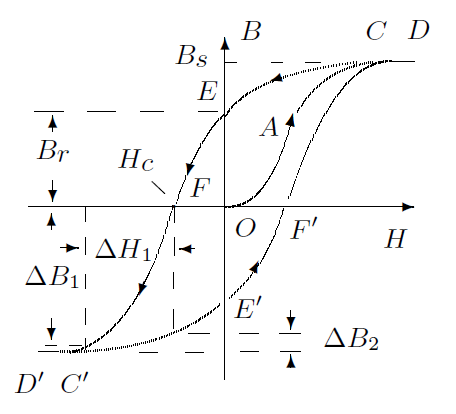
\includegraphics[width=41mm]{fig1.PNG}
\hfil
\caption{Петля гистерезиса ферромагнетика}
\label{figCurvesFF}
\end{floatingfigure}

Магнитная индукция \textbf{B} и напряжённость магнитного поля \textbf{H} в ферромагнетике неоднозначно связаны между собой: индукция зависит не только от напряжённости, но и от предыстории образца. В эксперименте будет исследоваться \textit{основная кривая намагничивания OACD} и \textit{предельная петля гистерезиса DEFD'E'F'D} (см. рис. 1).

С помощью баллистического гальванометра и амперметра будем косвенно измерять зависимость индукции магнитного поля от его напряжённости. \\
Напряжённость магнитного поля \textit{Н} в тороиде зависит от тока, текущего в намагничивающей обмотке:
\begin{equation}
    H = \frac{N_{T_0}}{\pi D}I,
\end{equation} 
где $D$ - средний диаметр тора, $N_{T_0}$ - количество витков.

Изменение поля приводит к изменению потока магнитной индукции Ф в сердечнике, в измерительной обмотке возникает ЭДС индукции, через гальванометр, в свою очередь, протекает импульс тока, изменяется положение рамки и, следовательно, зайчика. Окончательно (определив также баллистическую постоянную гальванометра, проведя измерения с соленоидом) для изменения магнитной индукции в сердечнике тороида получаем:
\begin{equation}
    \triangle B = \mu_0 (\frac{d_C}{d_T})^2 \frac{R}{R_1} \frac{N_C_0}{N_T_1} \frac{N_C_1}{l_C} \triangle I_1 \frac{\triangle x}{\triangle x_1},
\end{equation}
где $R$ - полное сопротивление измерительной цепи тороида, $d_C, d_T$ - диаметр поперечного сечения соленоида и тороида соответственно, $N_C_0$  - число витков пустотелого соленоида, $N_C_1$ - число витков короткой измерительной катушки $l_C$ - длина соленоида, $\triangle x_1$ - отклонение зайчика при работе с соленоидом, $\triangle x$ - отклонение зайчика в эксперименте.

\section{Экспериментальная установка}

\begin{figure}[h]
    \centering
    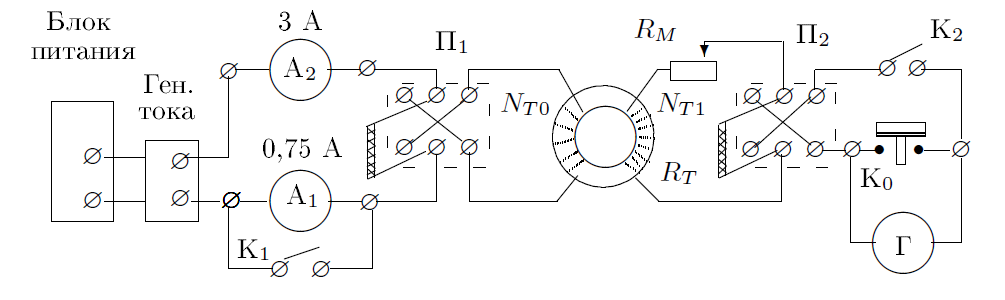
\includegraphics[width=10cm]{fig2.PNG}
    \caption{Схема установки для исследования петли гистерезиса}
    \label{fig:vac}
\end{figure}

\begin{figure}[h]
    \centering
    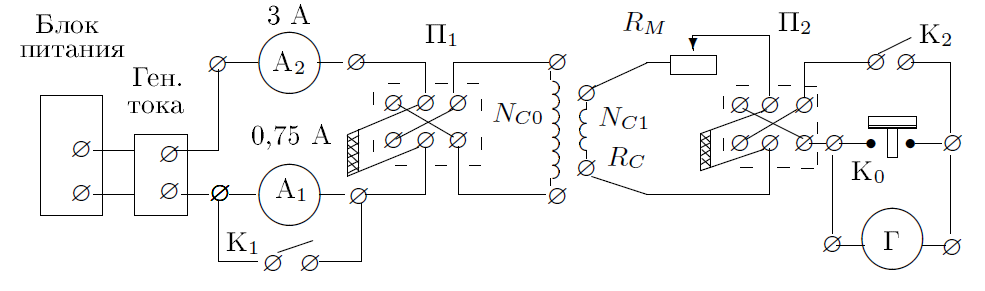
\includegraphics[width=10cm]{fig3.PNG}
    \caption{Схема установки для калибровки гальванометра}
    \label{fig:vac}
\end{figure}

После снятия петли гистерезиса необходимо размагнитить сердечник, подключив его к цепи переменного тока, постепенно снижая его амплитуду. Только затем следует приступать к снятию основной кривой намагничивания.

\section{Ход работы}

\begin{enumerate}
    \item Подготовив к работе экспериментальную установку, снимем зависимость величины скачка $\triangle x$ от величины силы тока в цепи $I$. Пройдём по всей петле гистерезиса, результаты занесём в таблицу 1.
    
    \begin{table}[h]
    \centering
    \begin{center}
    \caption{Зависимость $\triangle x$ от $I$ и соответствующие $H$ и $\triangle B$, петля гистерезиса}
    \end{center}
    \vspace{0.1cm}
    \label{tab:my_label}
    \begin{tabular}{ |p{1.2cm}||p{1cm}|p{1cm}|p{1cm}|p{1cm}|p{1cm}|p{1cm}|p{1cm}|p{1cm}|p{1cm}|p{1cm}|p{1cm}|p{1cm}| }
    \hline
        $I$, A & 1.73 & 0.94 & 0.58 & 0.49 & 0.40 & 0.36 & 0.325 & 0.284 & 0.246 & 0.187 & 0.11 & 0.0\\
\hline
    $\triangle x$, см & 0.0 & 15.9 & 9.2 & 3.3 & 2.5 & 2.8 & 1.5 & 1.0 & 0.9 & 1.5 & 2.0 & 3.0\\
\hline
    $H$, А/м & 9635.03 & 5242.20 & 3256.45 & 2715.29 & 2223.17 & 1982.40 & 1811.31 & 1582.80 & 1371.58 & 1039.97 & 613.61 & 0.0 \\
\hline
    $\triangle B$, Тл & 0.0 & 0.307 & 0.178 & 0.064 & 0.048 & 0.054 & 0.029 & 0.019 & 0.017 & 0.029 & 0.039 & 0.058\\
\hline
\hline

    $I$, А & 1.72 & 0.94 & 0.58 & 0.49 & 0.39 & 0.36 & 0.33 & 0.28 & 0.25 & 0.19 & 0.11 & 0\\
\hline
    $\triangle x$, см & 0.0 & 15.9 & 9.2 & 3.3 & 2.5 & 2.8 & 1.5 & 1.0 & 0.9 & 1.5 & 2 & 3 \\
\hline
    $H$, А/м & 9635.03 & 5242.2 & 3256.4 & 2715.3 & 2223.2 & 1982.4 & 1811.3 & 1582.8 & 1371.6 & 1039.9 & 613.6 & 0 \\
\hline 
    $\triangle B$, Тл & 0.205 & 0.25 & 0.38 & 0.37 & 0.46 & 0.28 & 0.30 & 0.39 & 0.24 & 0.45 & - & -\\
    
\hline
\hline

    $I$, мА & 0 & 0.11 & 0.187 & 0.25 & 0.28 & 0.32 & 0.36 & 0.40 & 0.49 & 0.58 & 0.94 & 1.73 \\
\hline
    $\triangle x$, см & - & 10.7 & 13.2 & 20.3 & 19.5 & 22.5 & 13.9 & 15.3 & 20.3 & 12.1 & 23.2 & 20.8 \\
\hline
    $H$, А/м & 0 & 613.06 & 1039.4 & 1372.7 & 1585.59 & 1809.6 & 1981.29 & 2222.05 & 2713.06 & 3253.7 & 5239.97 & 9633.36\\
\hline 
    $\triangle B$, Тл & 0.21 & 0.25 & 0.39 & 0.38 & 0.43 & 0.27 & 0.30 & 0.39 & 0.23 & 0.45 & 0.40 & - \\
\hline
\hline

    $I$, мА & 0.94 & 0.58 & 0.49 & 0.40 & 0.36 & 0.33 & 0.28 & 0.25 & 0.19 & 0.11 & 0.0 & - \\
\hline
    $\triangle x$, см & 16.1 & 8.9 & 3.5 & 3.5 & 1.9 & 2.5 & 1.1 & 1.1 & 1.5 & 2.5 & 5.2 & -\\
\hline
    $H$, А/м & 5241.64 & 3257.01 & 2714.73 & 2222.61 & 1982.96 & 1811.31 & 1582.80 & 1371.58 & 1039.97 & 613.06 & 0.0 & -\\
\hline
    $\triangle B$, Тл & 0.31 & 0.17 & 0.068 & 0.068 & 0.037 & 0.048 & 0.02 & 0.02 & 0.029 & 0.048 & 0.10 & -\\
\hline
\hline
    \end{tabular}
\end{table}
    
\item Отсоединим цепь от тороида, подсоединим её к пустотелому соленоиду. Откалибруем гальванометр. Получившиеся необходимые значения:

\begin{center}
    $I_{max}  = 1.2681 A$ \hspace{1cm} $\triangle x_{1} = 4.3$ см
\end{center}

\item Размагнитим тороид с помощью источника переменного тока и трансформатора. Снимем начальную кривую намагничивания, результаты занесём в таблицу 2.

   \begin{table}[h]
    \centering
    \begin{center}
    \caption{Зависимость $\triangle x$ от $I$ и соответствующие $H$ и $\triangle B$, начальная кривая намагничивания}
    \end{center}
    \vspace{0.1cm}
    \label{tab:my_label}
    \begin{tabular}{ |p{1.2cm}||p{1cm}|p{1cm}|p{1cm}|p{1cm}|p{1cm}|p{1cm}|p{1cm}|p{1cm}|p{1cm}|p{1cm}|p{1cm}|p{1cm}| }
 \hline
    $I$, мА & 0.11 & 0.19 & 0.25 & 0.28 & 0.32 & 0.36 & 0.40 & 0.49 & 0.58 & 0.94 & 1.73 & -\\
\hline
    $\triangle x$, см & 4.7 & 5.8 & 8.5 & 6.5 & 7.4 & 5.9 & 6.7 & 11.5 & 9.1 & 19.5 & 18.4 &  -\\
\hline
    $H$, А/м & 613.057 & 1039.41 & 1371.019 & 1581.69 & 1809.63 & 1981.29 & 2220.94 & 2712.5 & 3253.7 & 5236.62 & 9633.92 & - \\
\hline
    $\triangle B$, Тл & 0.09 & 0.11 & 0.16 & 0.126 & 0.143 & 0.114 & 0.129 & 0.22 & 0.18 & 0.38 & 0.36 & - \\
\hline
\hline

    \end{tabular}
\end{table}

\item В координатах $B(H)$ построим на одном графике петлю гистерезиса и начальную кривую намагничивания (рисунок 4).

\begin{figure}[h]
    \centering
    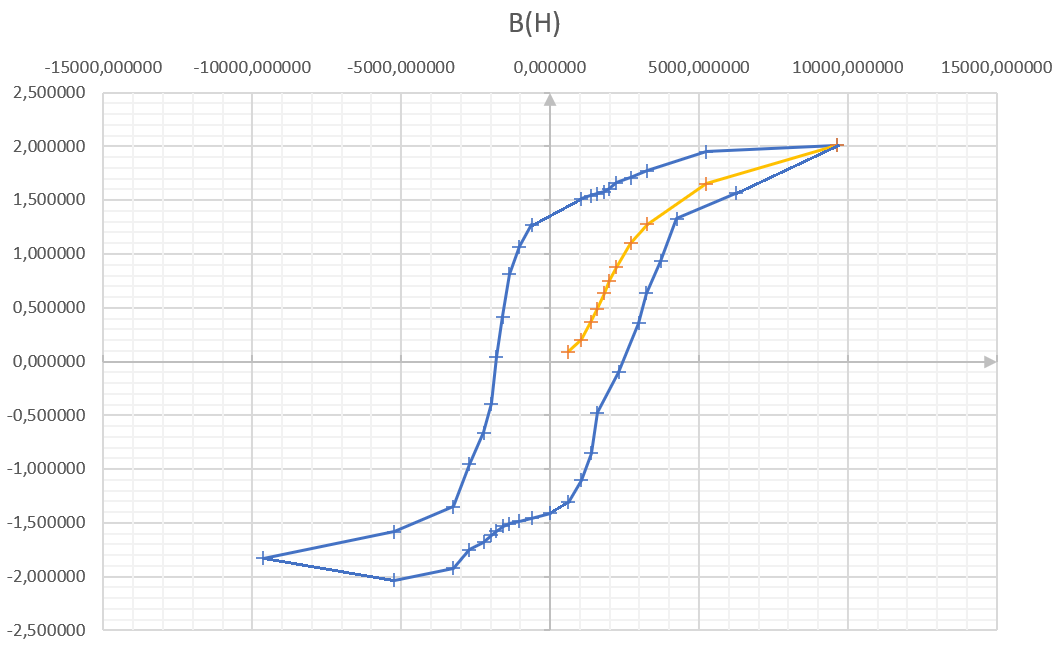
\includegraphics[width=\textwidth]{B(H).PNG}
    \caption{Петля гистерезиса и начальная кривая намагничивания для исследуемого образца}
    \label{fig:vac}
\end{figure}

По графику определим следующие величины и оценим их погрешности:
\begin{itemize}
    \item коэрцитивная сила $H_c$ - значение напряжённости магнитного поля, необходимое для полного размагничивания ферромагнитного вещества равна длине отрезка, высекаемого петлёй гистерезиса на горизонтальной оси. $H_c = 1809 \pm 193$ А/м.
    \item индукция насыщения $B_s$ -  максимально достижимое значение внутренней индукции магнитного материала при данной температуре. $B_s = 0.0080 \pm 0.0004$ Тл.
    \item максимальная дифференциальная магнитная проницаемость $\mu_d = \frac{1}{\mu_0}\frac{dB}{dH}$ - характеризующий связь между магнитной индукцией B и напряжённостью магнитного поля H в веществе. $\mu_d = 9715 \pm 270$
\end{itemize}

Итоговые результаты сведём в таблицу. Теоретические значения возьмём из справочника в пособии к лабораторным работам для технической стали.

   \begin{table}[h]
    \centering
    \begin{center}
    \caption{Соответствие теоретических и экспериментальных результатов}
    \end{center}
    \vspace{0.1cm}
    \label{tab:my_label}
    \begin{tabular}{ |p{2cm}||p{3cm}|p{3cm}| }
 \hline
     & Эксперимент & Справочник\\
\hline
\hline
     $H_c$, А/м & $1809 \pm 140$ & 70  \\
\hline
    $B_s$, Тл & $2.0 \pm 0.3$ & 2.15 \\
\hline
    $\mu_0$ & 1433 \pm 183$ & 5000 \\
\hline

    \end{tabular}
\end{table}

\section{Вывод}

В ходе работы были исследованы петля гистерезиса магнитомягкого материала, его начальная кривая намагничивания, экспериментально определены некоторые магнитные свойства. По кривой гистерезиса видно, что материал является магнитомягким, так как площадь петли мала. Также она симметрична и в целом соответствует теоретическим изображениям подобных кривых. Различие справочных и экспериментальных данных может объясняться тем, что, скорее всего, образец изготовлен не из чисто технического железа, а из сплава его с другим металлом. 

\end{enumerate}

\end{document}
